%%%%%%%%%%%%%%%%%%%%%%%%%%%%%%%%%%%%%%%%%%%%%%%%%%%%%%%%%%%%%%%%%%%%%%%%%%%%%%%
\chapter{Zero absoluto}
\label{Chap:ExpZeroAbsoluto}
%%%%%%%%%%%%%%%%%%%%%%%%%%%%%%%%%%%%%%%%%%%%%%%%%%%%%%%%%%%%%%%%%%%%%%%%%%%%%%%

\begin{fullwidth}\it
	Realizaremos um experimento em que verificaremos a pressão exercida por uma quantidade de gás com volume constante em função de sua temperatura. Através desses dados, determinaremos a temperatura para a qual teríamos uma pressão nula --- tal temperatura é o que denominamos como Zero Absoluto ---. Utilizaremos os seguintes conceitos/técnicas de análise de dados: medidas, algarismos significativos, gráficos, software para elaboração de gráficos, erros de escala e propagados, equação geral para o erro propagado, regressão linear, linearização, erros dos coeficientes $A$ e $B$, e planilhas para cálculo dos coeficientes $A$ e $B$ com erros.
\end{fullwidth}

%%%%%%%%%%%%%%%%%%%%%%%%%%%%%%%%%%%%%%%%%%%%%%%%%%%%%%%%%%%%%%%%%%%%%%%%%%%%%%%
\section{Termômetros}
%%%%%%%%%%%%%%%%%%%%%%%%%%%%%%%%%%%%%%%%%%%%%%%%%%%%%%%%%%%%%%%%%%%%%%%%%%%%%%%

Um método simples para verificar a temperatura é utilizar alguma propriedade de um material que varie com a temperatura como indicador de leitura. Muitos termômetros empregados rotineiramente em laboratórios usam mercúrio, outros usam álcool. Em ambos os casos, a propriedade que varia com a temperatura é o volume: o líquido de um reservatório se dilata e invade um tubo fino, onde a altura da coluna pode ser lida através de uma escala.

Outras propriedades podem ser utilizadas para verificar a temperatura, dentre elas a diferença de potencial elétrico entre uma junção bimetálica, a resistência elétrica de um material, o comprimento de uma fita metálica longa, a pressão de um volume confinado de um gás, etc. 

Em todos esses casos, é necessário se utilizar dois pontos para calibrar o termômetro com valores arbitrários de temperatura. A escala Celsius, por exemplo, utiliza a temperatura de fusão do gelo para zero graus e a temperatura de ebulição da água para 100 graus. No caso de um termômetro de mercúrio, podemos verificar a altura da coluna para a temperatura de fusão do gelo, realizando uma marca (na escala Celsius, \np[\tcdegree]{0}). Marcamos também a altura da coluna para a temperatura de ebulição da água (\np[\tcdegree]{100}). Dividimos então o intervalo entre essas duas marcas em um número de divisões menores. Podemos então verificar qualquer temperatura intermediária utilizando uma leitura da coluna de mercúrio. Podemos inclusive extrapolar as leituras para valores de temperatura maiores e menores que os extremos definidos pela temperatura de fusão do gelo e de ebulição da água, bastando para isso manter o tamanho da divisão igual às divisões intermediárias.

A confiabilidade das medidas de temperatura obtidas através de um termômetro está diretamente ligada à linearidade da propriedade observada com a variação da temperatura. Para faixas de temperatura relativamente pequenas, isso pode não ser um problema, mas se desejarmos realizar medições para uma ampla faixa de valores, comportamentos não-lineares podem ter efeito significativo. Além disso, se --- por exemplo --- desejarmos utilizar uma medida de temperatura extremamente elevada, não podemos utilizar um termômetro devido ao risco de danificá-lo\footnote{Nesse caso, podemos verificar a temperatura através do espectro da radiação emitida pelo corpo em questão.}. Portanto, é importante escolher um material e uma propriedade adequados à medida em questão.

%%%%%%%%%%%%%%%%%%%%%%%%%%%%%%%%%%%%%%%%%%%%%%%%%%
\subsection{Termômetros de gás a volume constante}
%%%%%%%%%%%%%%%%%%%%%%%%%%%%%%%%%%%%%%%%%%%%%%%%%%

Uma propriedade que pode ser utilizada para realizar uma medida confiável da temperatura é a pressão de um gás mantido em um volume constante. Segundo a equação dos gases ideais, a pressão varia com a temperatura de acordo com\footnote[][-1cm]{As temperaturas devem estar na escala Kelvin, discutida adiante.}
\begin{equation}
	PV = nRT,
\end{equation}
%
onde $R$ é a constante dos gases, $n$ é o número de moles de partículas do gás, $V$ é o volume ocupado pelo gás, e $T$ é a temperatura. Dessa equação, podemos escrever
\begin{equation}\label{Eq:PvsT}
	P = \frac{nR}{V} T.
\end{equation}

\begin{marginfigure}
\centering
\begin{tikzpicture}[>=Stealth]
    \draw[->] (0,0) -- (4,0) node[below left]{$T~(\tcdegree\rm{C})$};
    \draw[->] (0,0) -- (0,3) node[below left]{$P~(\rm{Pa})$};
    
    \draw[smooth,samples=10,domain=0:3.5]
    plot(\x,{tan(7)*\x + 3*tan(7)});
     \draw[dashed, smooth,samples=10,domain=0:3.5]
    plot(\x,{tan(14)*\x + 3*tan(14)});
     \draw[dashdotted, smooth,samples=10,domain=0:3.5]
    plot(\x,{tan(20)*\x + 3*tan(20)});
   
\end{tikzpicture}
\caption{Para um gás real, a relação entre $P$ e $T$ depende do gás, porém é sempre linear.\label{Fig:RelPressaoTempGasIdeal}}
\end{marginfigure}

Para um gás real, a relação entre a pressão e a temperatura depende do tipo de gás utilizado. Porém, se o gás estiver a baixa pressão, ou seja, estiver \emph{rarefeito}, e a temperatura a ser medida for maior que aquela em que o gás se torna um líquido, podemos utilizar qualquer gás para realizar medidas de temperatura. A diferença entre diversos gases será a inclinação da reta, porém as relações serão sempre lineares (Figura~\ref{Fig:RelPressaoTempGasIdeal}).

Para um gás mantido a um volume $V$ constante em um reservatório hermético, podemos afirmar que o número de moles $n$ se mantém constante. Temos então uma relação de proporcionalidade entre a pressão do gás e a temperatura a que ele se encontra. Um dispositivo que utiliza essa propriedade para realizar medidas é denominado \emph{termômetro de gás a volume constante}.

\begin{marginfigure}
\centering
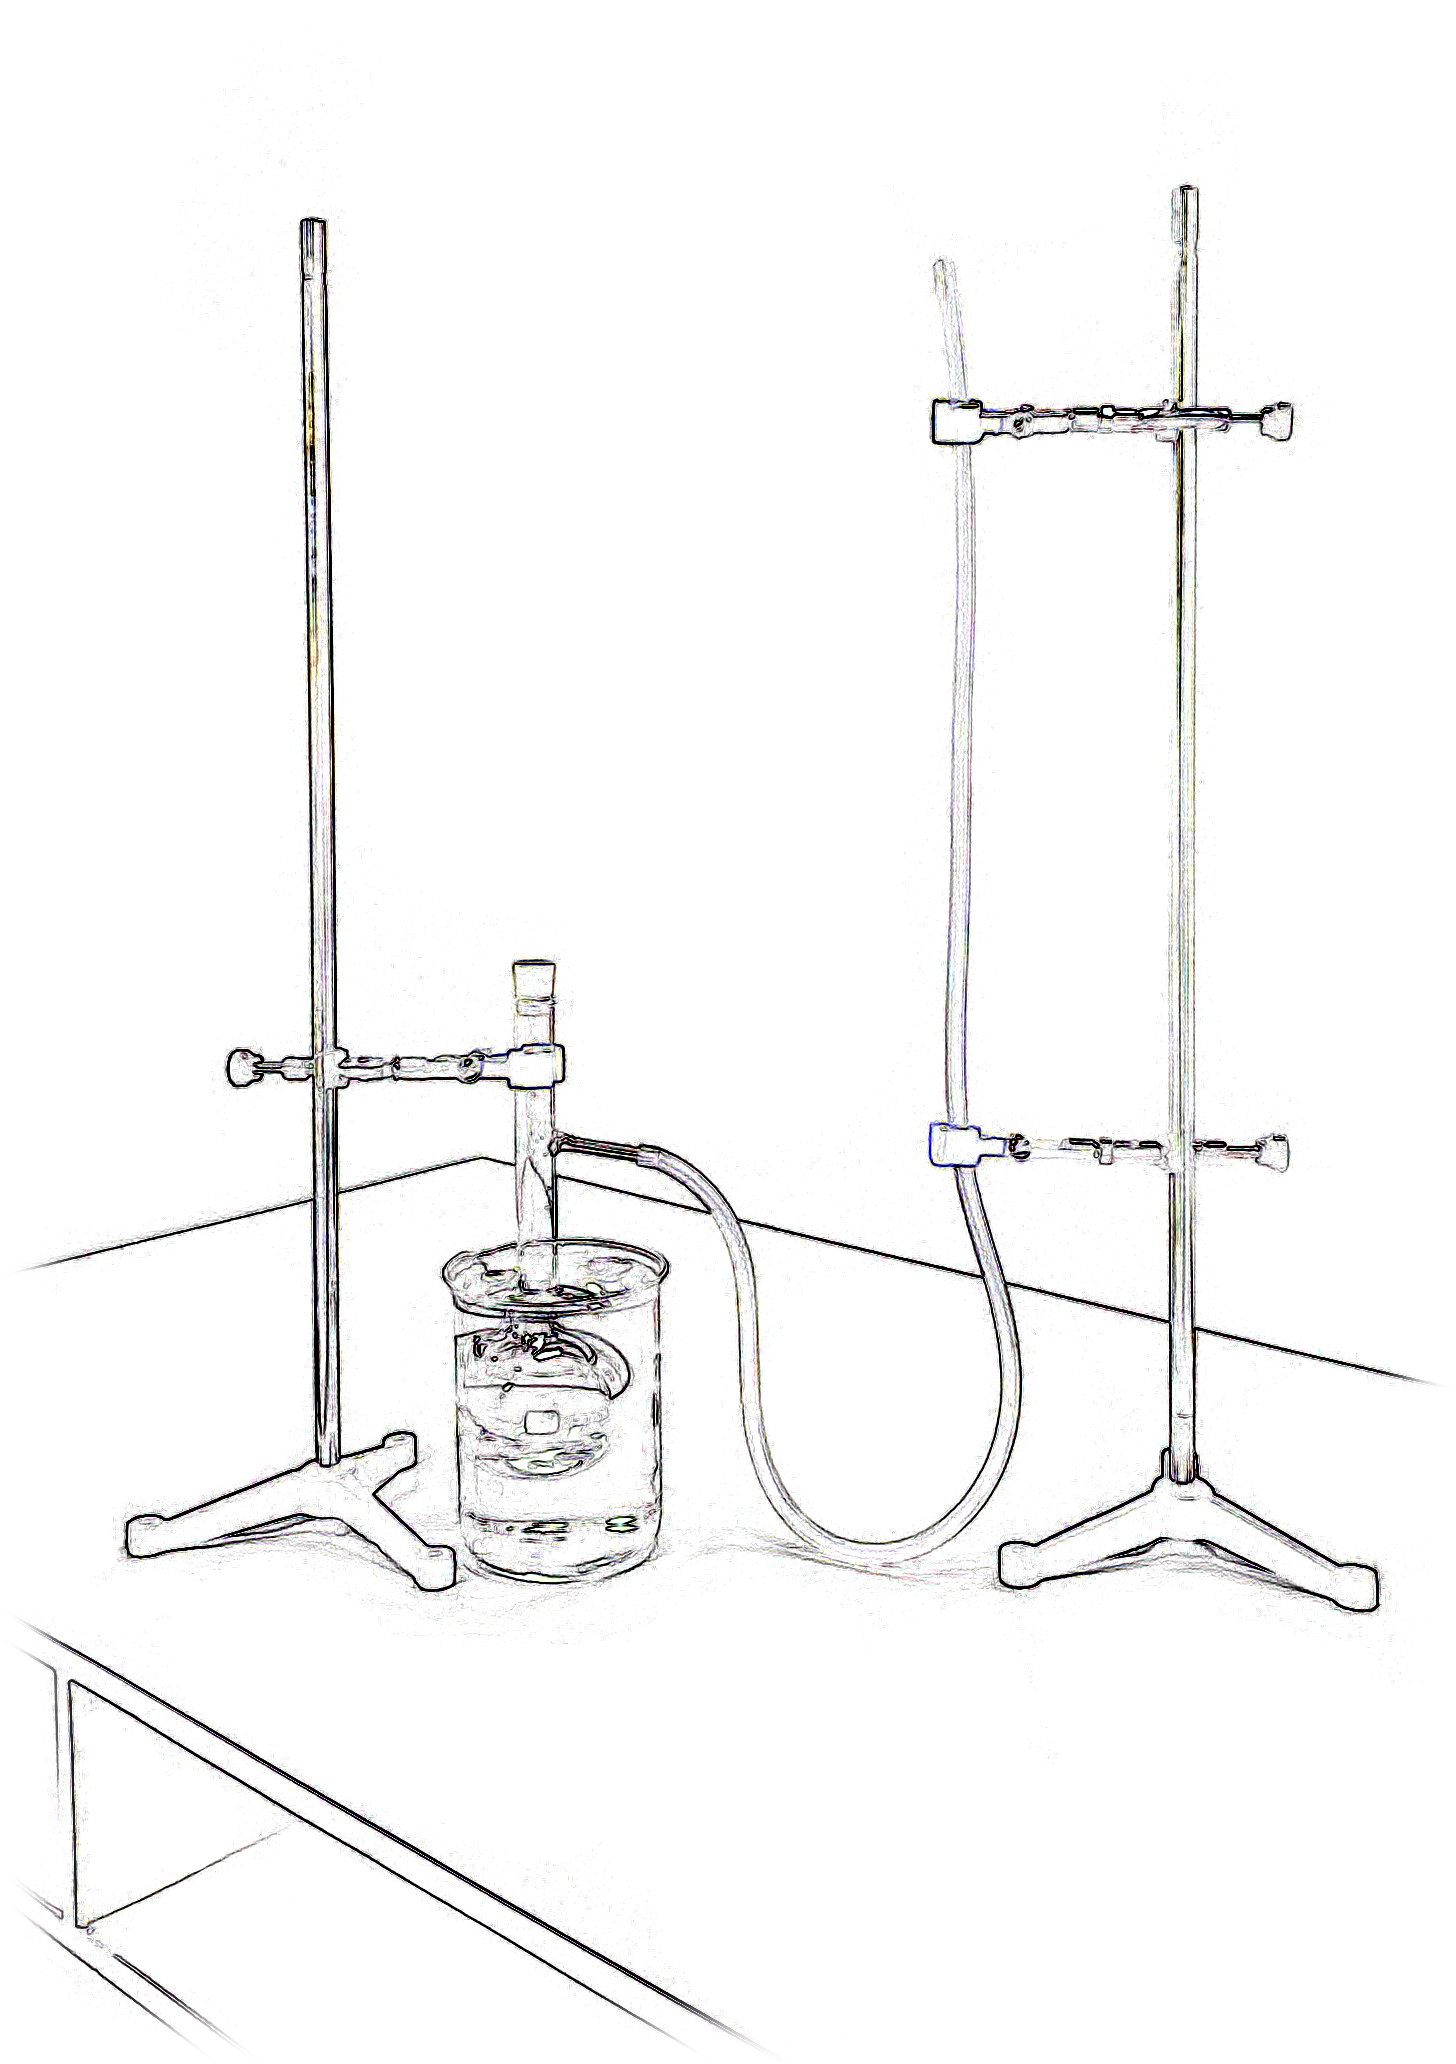
\includegraphics[width=\textwidth]{Ilustrations/Term_gas.png}
\caption{Termômetro de gás a volume constante.\label{Fig:TermometroGas}}
\end{marginfigure}

A Figura~\ref{Fig:TermometroGas} mostra um desenho esquemático de um dispositivo desse tipo: nela temos um balão de destilação fechado com uma rolha e em cuja saída lateral está conectada um tubo flexível, sendo que a outra extremidade é aberta. Dentro do tubo temos um fluido de densidade conhecida. O balão fica submerso em um banho térmico cuja temperatura estamos interessados em medir.

Como a extremidade livre do tubo é aberta, ela está sujeita à pressão atmosférica, logo, a pressão do gás dentro do balão será determinada pela soma da pressão atmosférica com a pressão exercida pela coluna de líquido:
\begin{equation}\label{Eq:PressaoColunaFluido}
	P = P_0 + \rho g h,
\end{equation}
%
onde $P_0$ é a pressão atmosférica, $\rho$ é a densidade do fluido dentro do tubo, $g$ é a aceleração da gravidade e $h$ é a altura\footnote{Note que $h$ é a \emph{altura} da coluna, não seu comprimento. Tal distância deve ser medida \emph{verticalmente}.} (veja a Figura~\ref{Fig:FigEsquematicaTermGas}).

Para determinarmos o valor da altura da coluna de fluido adequadamente, devemos nos certificar que o volume de gás dentro do balão seja mantido constante. Para isso, devemos verificar a posição da coluna de fluido na extremidade do tubo que está ligada ao balão e marcarmos sua posição para referência futura (tal marca é representada pela seta na Figura~\ref{Fig:FigEsquematicaTermGas}). Ao aquecermos o gás, o fluido no tubo se deslocará devido à pressão exercida sobre ele, fazendo com que as posições dos topos das colunas em ambas as extremidades do tubo  mudem de posição. Para que o gás volte ao volume inicial, o topo da coluna da extremidade do tubo ligada ao balão deve voltar ao nível original, o que pode ser feito deslocando a extremidade livre para cima. Só então devemos aferir a distância vertical $h$ entre as colunas.

\begin{marginfigure}[-4cm]
\centering
\begin{tikzpicture}[>=Stealth,
interface/.style={
        % superfície
        postaction={draw,decorate,decoration={border,angle=-45,
                    amplitude=0.2cm,segment length=2mm}}}
    ]
    
    \draw[pattern = north west lines] (-1,1.5) -- (-1, 0) -- (1,0) -- (1,1.5) -- (0.9,1.5) -- (0.9,0.1) -- (-0.9,0.1) -- (-0.9, 1.5) -- cycle;
    
    % balão
    \draw (0,0.75)+(95:0.5) arc[radius = 0.5, start angle = -265, end angle = 85];
    \draw (0,0.75)++(95:0.5) -- +(0,1) coordinate (be);
    \draw (0,0.75)++(85:0.5) -- +(0,0.5) coordinate (li);
    \draw (li) ++(0,0.05) coordinate (ls) -- +(0,0.45) coordinate (bd);
    \draw (li) -- +(-5:0.3) coordinate (si);
    \draw (ls) -- +(-5:0.3);
    \draw[fill] (0,2.25)+(-0.05,0) rectangle +(0.05,0.1);
    \node (P) at (0,0.75) {$P$};
    
    % mangueira
    \draw[double = white, double distance = 0.05cm] (si)+(0,0.025) .. controls (1,1.65) and (1.5,2) .. (1.5,1);
    
    % tubo em U
    \draw (1.475, 1) -- (1.475, 0.25) arc[start angle = -180, end angle = 0, radius = 0.2] -- +(0,2);
    \draw (1.525, 1) -- (1.525, 0.25) arc[start angle = -180, end angle = 0, radius = 0.15] -- +(0,2);
    \draw[fill] (1.475, 0.75) -- (1.475, 0.25) arc[start angle = -180, end angle = 0, radius = 0.2] -- ++(0,1) -- ++(-0.05,0) -- ++(0,-1) arc[start angle = 0, end angle = -180, radius = 0.15] -- ++(0,0.5) -- cycle;  
    
    % marca de referência
    \draw[->] (1.2, 0.75) -- (1.455,0.75);
    
    % altura da coluna
    \draw[dotted] (1.455,0.75) -- (2.2,0.75);
    \draw[dotted] (1.875,1.25) -- (2.2,1.25);
    \draw[->] (2.2, 0.25) -- (2.2, 2.25) node[below right]{$y$};
    \draw[|-|] (2.2,0.75) node[right]{$0$} -- (2.2,1.25) node[right]{$y = h$};
    
    % líquido
    \draw[pattern = dots] (0,0.75)+(95:0.5) arc[radius = 0.5, start angle = -265, end angle = 85] -- ++(0,0.15) -- (0.9, 1.4) -- (0.9,0.1) -- (-0.9,0.1) -- (-0.9,1.4) -- (-0.044,1.4) -- cycle;
    
    % mesa
    \draw[interface] (-1.25,0) -- (3.25,0);
    
\end{tikzpicture}
\caption{A pressão do gás pode ser determinada pela soma da pressão atmosférica com a pressão exercida pela coluna d'água cuja altura é $h$. O gás deve ser mantido a volume constante, o que implica que a coluna d'água na extremidade do tubo ligado ao balão deve ser mantida na marca de referência indicada pela flecha.\label{Fig:FigEsquematicaTermGas}}
\end{marginfigure}

\begin{marginfigure}[2cm]
\centering
\begin{tikzpicture}[>=Stealth]
    \draw[->] (0,0) -- (4,0) node[below left]{$h$};
    \draw[->] (0,0) -- (0,3.5) node[below left]{$T$};
    
    \draw (0,1) -- (3.5,3);
    \draw[dotted] (0.75,0) node[below]{$h_f$} -- (0.75, 1.43) -- (0, 1.43) node[left]{$T_f$};
    \draw[dotted] (3,0) node[below]{$h_e$} -- (3, 2.71) -- (0, 2.71) node[left]{$T_e$};
   
\end{tikzpicture}
\caption{A relação entre a temperatura $T$ e a altura $h$ é linear, o que nos permite utilizá-la como a escala de um termômetro.}
\end{marginfigure}

Como sabemos que existe uma relação linear da temperatura com a pressão, e uma relação linear da pressão com a altura $h$ da coluna, podemos determinar uma relação linear entre a temperatura $T$ e a altura $h$: de acordo com a Equação~\eqref{Eq:PvsT}, podemos escrever
\begin{equation}
    T = \frac{V}{nR} P,
\end{equation}
%
ou, usando a Equação~\eqref{Eq:PressaoColunaFluido},
\begin{align}
    T &= \frac{V}{nR} (P_0 + \rho g h) \\
    &= \frac{VP_0}{nR} + \frac{V\rho g}{nR}h.
\end{align}

Para que possamos definir valores numéricos específicos de temperatura, precisamos de duas temperaturas de referência, como as de fusão e ebulição da água, por exemplo. Uma vez determinados os valores arbitrários de temperatura $T_f$ e $T_e$ e as alturas $h_f$ e $h_e$ correspondentes a tais temperaturas, podemos determinar a relação entre $T$ e $h$ considerando que a tal relação é linear, o que implica em uma forma dada por
\begin{equation}
    T = Bh + A,
\end{equation}
%
onde
\begin{equation}
\begin{system} B h_e + A &= T_e \\ B h_f + A &= T_f. \end{system}
\end{equation}
%
Resolvendo esse sistema, obtemos
\begin{align}
    B &= \frac{T_e - T_f}{h_e - h_f} \\
    A &= T_f - \frac{T_e - T_f}{h_e - h_f} h_f,
\end{align}
%
de onde obtemos
\begin{equation}
    T = (h - h_f)\frac{T_e - T_f}{h_e - h_f} + T_f.
\end{equation}
 
%%%%%%%%%%%%%%%%%%%%%%%%%%
\subsection{Zero absoluto}
%%%%%%%%%%%%%%%%%%%%%%%%%%

Para qualquer gás utilizado no termômetro, a medida que a temperatura diminui, a pressão do gás também diminui. Essa relação deve ter um valor para o qual a pressão exercida pelo gás é nula, correspondendo a uma temperatura mínima ou um \emph{zero absoluto} para a escala de temperatura. Apesar de a inclinação das retas de $P \times T$ serem diferentes para gases diferentes, o valor para o qual a pressão é zero é o mesmo para qualquer gás, sendo que tal valor é determinado experimentalmente, correspondendo na escala Celsius a $T_0^C = -\np[\tcdegree C]{273,15}$.

\begin{figure}\forceversofloat
\centering
\begin{tikzpicture}[>=Stealth]
    \draw[->] (-3.5,0) -- (4,0) node[below left]{$T~(\tcdegree\rm{C})$};
    \draw[->] (0,0) -- (0,3) node[below left]{$P~(\rm{Pa})$};
    
    \draw[smooth,samples=100,domain=0:3.5]
    plot(\x,{tan(7)*\x + 3*tan(7)});
     \draw[dashed, smooth,samples=100,domain=0:3.5]
    plot(\x,{tan(14)*\x + 3*tan(14)});
     \draw[dashdotted, smooth,samples=100,domain=0:3.5]
    plot(\x,{tan(20)*\x + 3*tan(20)});
   
   \draw[dotted, smooth,samples=100,domain=-3:0]
    plot(\x,{tan(7)*\x + 3*tan(7)});
     \draw[dotted, smooth,samples=100,domain=-3:0]
    plot(\x,{tan(14)*\x + 3*tan(14)});
     \draw[dotted, smooth,samples=100,domain=-3:0]
    plot(\x,{tan(20)*\x + 3*tan(20)});
   
   \draw[fill] (-3,0) circle (1pt) node[below] {$T_0^C$};
\end{tikzpicture}
\caption{Extrapolando a relação entre $P$ e $T$ para qualquer gás, obtemos sempre o mesmo valor de temperatura para o qual a pressão será nula. No caso da escala Celsius, tal valor corresponde a $T_0^C = \np[\tcdegree C]{-273.15}$.}
\end{figure}

Podemos então utilizar o valor do zero absoluto para definir uma escala de temperaturas --- a escala Kelvin --- em que a menor temperatura possível seja zero, correspondendo ao zero absoluto, e na qual a temperatura de fusão do gelo seja \np[K]{273,15}, sendo que a relação entre tal escala e a escala Celsius será dada por
\begin{equation}\label{Eq:RelKC}
	T_K = T_C + \np{273.15}.
\end{equation}

De acordo com a interpretação cinética para os gases, a pressão exercida pelo gás está relacionada à energia cinética das partículas que o compõe: a pressão é exercida nas paredes de um recipiente pelas colisões sucessivas das partículas. Ao se atingir o zero absoluto, a pressão e a energia cinética serão nulas\footnote{Se não há pressão, isso só pode ser explicado pela ausência de colisões entre as partículas do gás e as paredes do recipiente, o que implica que as partículas estão em repouso em relação ao recipiente e que ---~consequentemente~--- suas energias cinéticas são nulas.}, o que corresponderia classicamente a todas as partículas do gás repousarem no fundo do recipiente que as contém.

%%%%%%%%%%%%%%%%%%%%%%%%%%%%%%%%%%%%%%%%%%
\subsection{Determinação do zero absoluto}
%%%%%%%%%%%%%%%%%%%%%%%%%%%%%%%%%%%%%%%%%%

Se tomarmos um termômetro de gás a volume constante como o da Figura~\ref{Fig:TermometroGas}, podemos determinar o valor do zero absoluto com o auxílio de um segundo termômetro. Para isso, basta tomarmos dados da pressão do gás no balão, em função da temperatura do banho térmico no qual o balão está submerso.

Para isso, observamos que ---~através da expressão para a pressão de um gás ideal e da Equação~\eqref{Eq:RelKC} entre as temperaturas na escala Kelvin e na escala Celsius~--- obtemos a seguinte relação:
\begin{align}
    PV &= nRT_K \\
    &= nR(T_C + T_0) \\
    &= nRT_C + nRT_0,
\end{align}
%
onde $T_0$ corresponde à diferença entre as escalas Celsius e Kelvin, o que corresponde a \np{273.15}. Podemos então escrever a relação
\begin{equation}
    P = \frac{nR}{V}T_C + \frac{nR}{V}T_0.
\end{equation}
%
Se o volume $V$ do gás é mantido constante, a expressão acima segue um comportamento linear. Comparando-a à equação da reta $y = Bx + A$, verificamos que
\begin{align}
    B &= \frac{nR}{V} \\
    A &= \frac{nR}{V}T_0,
\end{align}
%
de onde obtemos
\begin{equation}\label{Eq:EqRazaoABZeroAbs1}
    T_0 = \frac{A}{B}.
\end{equation}
%
Ao verificarmos os valores de pressão $P$ em função da temperatura $T$ utilizando o aparato da Figura~\ref{Eq:RelKC}, podemos determinar os valores de $A$ e $B$, de onde podemos calcular o valor do zero absoluto na escala Celsius experimentalmente, um vez que 
\begin{equation}\label{Eq:EqRazaoABZeroAbs2}
    T_0^C = - T_0.
\end{equation}

%%%%%%%%%%%%%%%%%%%%%%%%%%%%%%%%%%%%%%%%%%%%%%%%%%%%%%%%%%%%%%%%%%%%%%%%%%%%%%%
\section{Experimento}
%%%%%%%%%%%%%%%%%%%%%%%%%%%%%%%%%%%%%%%%%%%%%%%%%%%%%%%%%%%%%%%%%%%%%%%%%%%%%%%

%%%%%%%%%%%%%%%%%%%%%%
\subsection{Objetivos}
\label{Sec:ObjetivosZeroAbsoluto}
%%%%%%%%%%%%%%%%%%%%%%

\begin{itemize}
	\item Verificar que a relação entre a pressão de um gás com a temperatura é linear.
	\item Calcular o valor do zero absoluto na escala Celsius.
\end{itemize}

%%%%%%%%%%%%%%%%%%%%%%%%%%%%%%%%%%%%%%%%%%%%%%%%%%%%%%%%%%%%%%%%%%%%%%%%%%%%%%%
\section{Material Necessário}
%%%%%%%%%%%%%%%%%%%%%%%%%%%%%%%%%%%%%%%%%%%%%%%%%%%%%%%%%%%%%%%%%%%%%%%%%%%%%%%

\begin{multicols}{2}
\begin{itemize}
	\item Becker;
	\item Balão de destilação com saída lateral;
	\item Rolha;
	\item Suporte vertical com garras;
	\item Termômetro;
	\item Tubo flexível transparente longo;
	\item Réguas e trenas;
	\item Bastão de vidro;
	\item Recipiente com água;
	\item Tela de amianto e suporte para a tela;
	\item Lamparina e fósforos;
	\item Flanela.
\end{itemize}
\end{multicols}

\begin{figure}[!h]
\centering
\forceversofloat
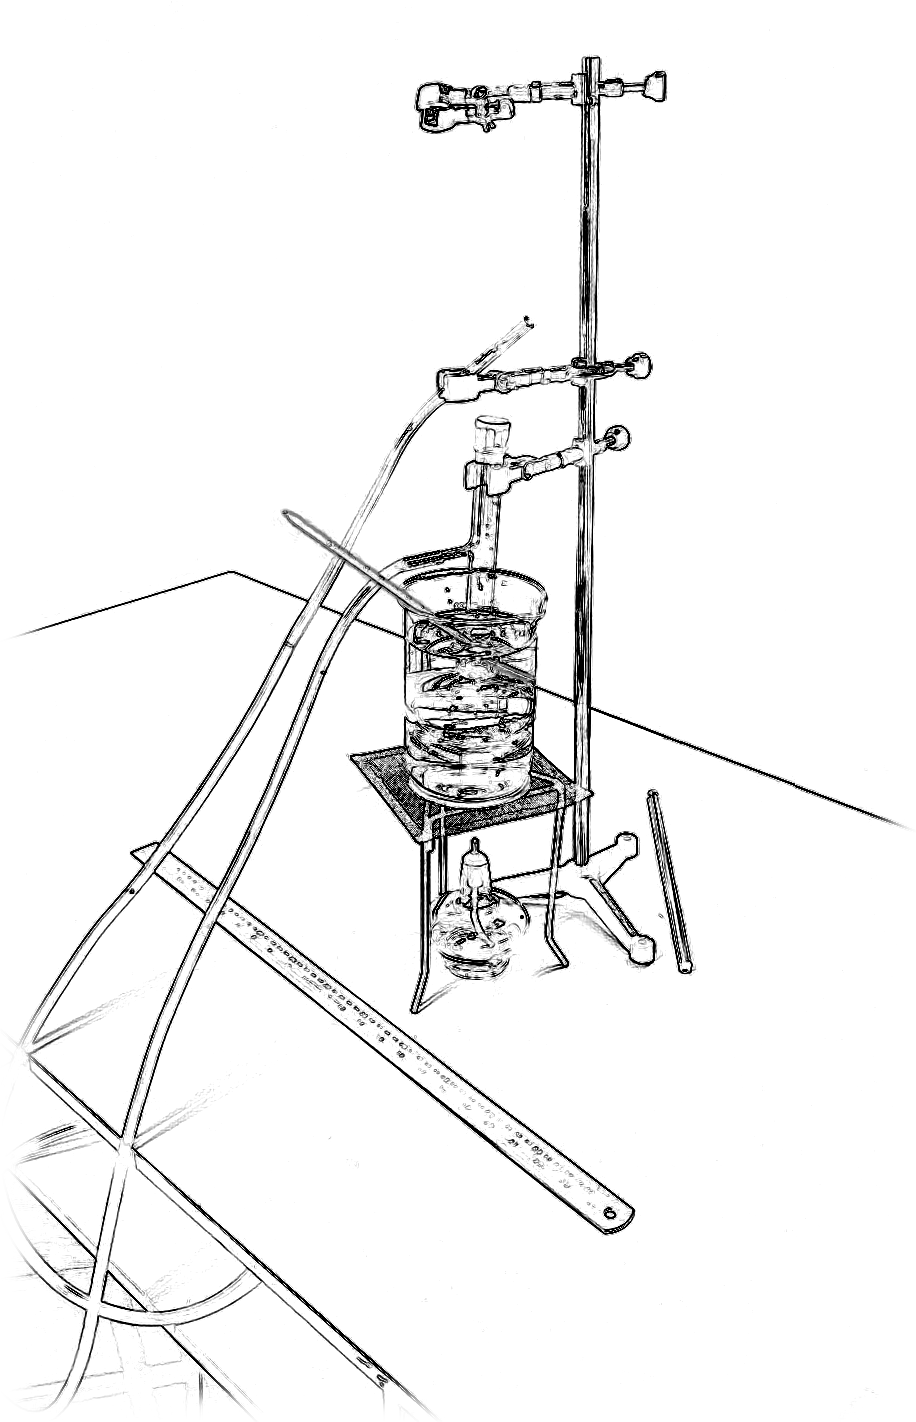
\includegraphics[width=0.7\textwidth]{Ilustrations/AparatoZeroAbs.png}
\caption{Aparato para a verificação do zero absoluto.}
\end{figure}
%%%%%%%%%%%%%%%%%%%%%%%%%%%%%%%%%%%%%%%%%%%%%%%%%%%%%%%%%%%%%%%%%%%%%%%%%%%%%%%
\section{Procedimento Experimental}
%%%%%%%%%%%%%%%%%%%%%%%%%%%%%%%%%%%%%%%%%%%%%%%%%%%%%%%%%%%%%%%%%%%%%%%%%%%%%%%

%%%%%%%%%%%%%%%%%%%%%%%%%%%%%%%%
\subsection{Montagem do aparato}
%%%%%%%%%%%%%%%%%%%%%%%%%%%%%%%%

\begin{enumerate}
\item Disponha a tela de amianto sobre o suporte e coloque o becker sobre ela;
\item Disponha o suporte vertical próximo ao becker. Afixe nele uma garra e a utilize para segurar o balão de destilação. A parte arredondada do balão deve ficar disposta dentro do becker, porém sem tocar o fundo;
\item Adicione água ao tubo de forma que ele fique sem bolhas e com água até aproximadamente \np[cm]{20} de cada extremidade;
\item Prenda o tubo ao suporte com o auxílio de garras de forma que uma das extremidades possa ser presa ao balão e que a outra fique à mesma altura que a primeira (a parte restante do tubo deve ficar abaixo da mesa, no chão);
\item Prenda uma das extremidades do tubo à saída lateral do balão de destilação;
\item Se o balão estiver com a extremidade superior aberta, feche-a com a rolha;
\item Adicione água ao becker até cobrir a parte arredondada do balão e parte do gargalo;
\end{enumerate}

%%%%%%%%%%%%%%%%%%%%%%%%%%%%%%%%%%%%%%%%%%%
\subsection{Coleta dos dados experimentais}
%%%%%%%%%%%%%%%%%%%%%%%%%%%%%%%%%%%%%%%%%%%

\begin{enumerate}
\item Verifique a pressão atmosférica $P_0$ e a anote na Tabela~\ref{Tab:Dados};
\item Verifique a temperatura da água com o termômetro e a anote na Tabela~\ref{Tab:Dados}.
\item Verifique a \emph{distância vertical}\footnote{Veja a Figura~\ref{Fig:FigEsquematicaTermGas}.} $h$ entre os topos das colunas d'água nas duas extremidades da mangueira (Veja a Figura~\ref{Fig:FigEsquematicaTermGas}) e a anote na Tabela~
\ref{Tab:Dados}.\footnote{Se a altura da coluna na extremidade do tubo ligada ao balão for maior que a da coluna na extremidade livre, o valor de $h$ deve ser marcado com um sinal negativo, pois a pressão no balão é menor que a atmosférica.}
\item Na extremidade do tubo ligada ao balão, marque com caneta a posição do topo da coluna d'água. Essa marca é importante pois ao tomarmos medidas da distância vertical $h$ precisamos garantir que o gás é mantido a volume constante.
\item Disponha a lamparina abaixo da tela de amianto e a acenda.
\item Agite a água constantemente com o bastão de vidro para que ela tenha uma temperatura homogênea; 
\item Assim que a temperatura aumentar \np[\tcdegree C]{2}, levante a extremidade livre do tubo de forma que o nível na extremidade ligada ao balão volte à posição original, marcada no passo anterior. Verifique o valor da temperatura\footnote{Meça a temperatura próximo da metade da parte arredondada do balão, visando evitar possíveis regiões de temperatura não uniforme (o ideal é apagar a lamparina e agitar a água por alguns segundos, anotando a temperatura atingida no equilíbrio térmico).} e a diferença vertical $h$ entre as colunas d'água e anote na Tabela~\ref{Tab:Dados}.
\item Aguarde até que a temperatura volte a subir \np[\tcdegree C]{2,0}, reajuste o nível da coluna d'água na extremidade do tubo ligada ao balão até que ele volte a coincidir com a marca inicial, e determine o novo valor de $h$. Anote os novos valores na Tabela~\ref{Tab:Dados}.
\item Repita o processo do item anterior de forma a obter o maior número de dados experimentais possível, ou completar a Tabela~\ref{Tab:Dados}.
\end{enumerate}

%%%%%%%%%%%%%%%%%%%%%%%%%%%%%%%%%%%%%%%%%%%%%%%%%%%%%%%%%%%%%%%%%%%%%%%%%%%%%%%
%%%%%%%%%%%%%%%%%%%%%%%%%%%%%%%%%%%%%%%%%%%%%%%%%%%%%%%%%%%%%%%%%%%%%%%%%%%%%%%
%%%%%%%%%%%%%%%%%%%%%%%%%%%%%%%%%%%%%%%%%%%%%%%%%%%%%%%%%%%%%%%%%%%%%%%%%%%%%%%
%%%%%%%%%%%%%%%%%%%%%%%%%%%%%%%%%%%%%%%%%%%%%%%%%%%%%%%%%%%%%%%%%%%%%%%%%%%%%%%
\cleardoublepage

\noindent{}{\huge\textit{Zero absoluto}}

\vspace{15mm}

\begin{fullwidth}
\noindent{}\makebox[0.6\linewidth]{Turma:\enspace\hrulefill}\makebox[0.4\textwidth]{  Data:\enspace\hrulefill}
\vspace{5mm}

\noindent{}\makebox[0.6\linewidth]{Aluno(a):\enspace\hrulefill}\makebox[0.4\textwidth]{  Matrícula:\enspace\hrulefill}

\noindent{}\makebox[0.6\linewidth]{Aluno(a):\enspace\hrulefill}\makebox[0.4\textwidth]{  Matrícula:\enspace\hrulefill}

\noindent{}\makebox[0.6\linewidth]{Aluno(a):\enspace\hrulefill}\makebox[0.4\textwidth]{  Matrícula:\enspace\hrulefill}

\noindent{}\makebox[0.6\linewidth]{Aluno(a):\enspace\hrulefill}\makebox[0.4\textwidth]{  Matrícula:\enspace\hrulefill}

\noindent{}\makebox[0.6\linewidth]{Aluno(a):\enspace\hrulefill}\makebox[0.4\textwidth]{  Matrícula:\enspace\hrulefill}
\end{fullwidth}

\vspace{5mm}

%%%%%%%%%%%%%%%%%%%%%%%%%%%%%%%%%%%%%%%%%%%%%%%%%%%%%%%%%%%%%%%%%%%%%%%%%%%%%%%
\section{Questionário}
%%%%%%%%%%%%%%%%%%%%%%%%%%%%%%%%%%%%%%%%%%%%%%%%%%%%%%%%%%%%%%%%%%%%%%%%%%%%%%%

\begin{question}[type={exam}]{1}
Apresente os resultados de maneira clara e organizada. Mostre os cálculos requisitados de maneira clara e sucinta, evidenciando o raciocínio desenvolvido.
\end{question}

\begin{question}[type={exam}]{1}
Liste os equipamentos utilizados. Para os instrumentos de medida, descreva o tipo do equipamento, sua resolução, e seu erro de escala.
\end{question}

\begin{question}[type={exam}]{1}
Preencha as tabelas com o número adequado de algarismos significativos, unidades, e erros de escala apropriados. 
\end{question}

\begin{question}[type={exam}]{1.5}
Elabore um gráfico de $P \times T$ para os dados da Tabela~\ref{Tab:Dados}.
\end{question}

\begin{question}[type={exam}]{1}
Calcule a reta que melhor representa os dados experimentais utilizando o método dos mínimos quadrados e a adicione ao gráfico.
\end{question}

\begin{question}[type={exam}]{1}
Utilizando as Equações~\ref{Eq:EqRazaoABZeroAbs1} e~\ref{Eq:EqRazaoABZeroAbs2} e os coeficientes para a regressão linear obtidos através do método de mínimos quadrados, calcule o valor de temperatura para o qual a pressão será zero. Verifique o erro percentual entre tal valor de temperatura e o valor de referência $T_0^{\textrm{ref}} = -\np[\tcdegree C]{273,15}$ através da expressão
\begin{equation}
	E_{\%} = \left|\frac{x-x_{\textrm{ref}}}{x_{\textrm{ref}}}\right| \times 100.
\end{equation}
\end{question}

\begin{question}[type={exam}]{2}
Calcule os erros associados aos coeficientes $A$ e $B$ da regressão linear e ---~a partir dos coeficientes, dos erros a eles associados, e das Equações~\ref{Eq:EqRazaoABZeroAbs1} e~\ref{Eq:EqRazaoABZeroAbs2}~---  calcule o erro associado a $T_C^0$.
\end{question}

\begin{question}[type={exam}]{1.5}
Considerando os objetivos do experimento, listados na Seção~\ref{Sec:ObjetivosZeroAbsoluto}, e os resultados obtidos nas questões anteriores, discuta quais objetivos foram atingidos com sucesso, justificando suas conclusões. Se algum objetivo não foi atingido, discuta quais são os possíveis motivos do fracasso e que providências podem ser tomadas para que eles sejam alcançados.
\end{question}

%%%%%%%%%%%%%%%%%%%%%%%%%%%%%%%%%%%%%%%%%%%%%%%%%%%%%%%%%%%%%%%%%%%%%%%%%%%%%%%
\section{Tabelas}
%%%%%%%%%%%%%%%%%%%%%%%%%%%%%%%%%%%%%%%%%%%%%%%%%%%%%%%%%%%%%%%%%%%%%%%%%%%%%%%

\begin{table*}[!htb]
\caption{Dados para a altura da coluna de água em função da temperatura.}
\label{Tab:Dados}
	\begin{center}
		\begin{tabular}{cp{45mm}p{45mm}p{45mm}c}
		\toprule
		&\multicolumn{2}{l}{\textbf{Constantes}}\\
		\cmidrule{2-3}
		& \cellcolor[gray]{0.89} $P_0$ &\cellcolor[gray]{0.92} \\
		& \cellcolor[gray]{0.95} $\rho$ & \cellcolor[gray]{0.97}\\
		\cmidrule{2-3}
		\\
		&\multicolumn{2}{l}{\textbf{Dados para a altura da coluna}} \\
		\cmidrule{2-4}
		& $T$ & $h$ & $P$ & \\
		\cmidrule{2-4}
		& \cellcolor[gray]{0.89} & \cellcolor[gray]{0.92} & \cellcolor[gray]{0.89} \\
		& \cellcolor[gray]{0.95} & \cellcolor[gray]{0.97} & \cellcolor[gray]{0.95} \\
		& \cellcolor[gray]{0.89} & \cellcolor[gray]{0.92} & \cellcolor[gray]{0.89} \\
		& \cellcolor[gray]{0.95} & \cellcolor[gray]{0.97} & \cellcolor[gray]{0.95} \\
		& \cellcolor[gray]{0.89} & \cellcolor[gray]{0.92} & \cellcolor[gray]{0.89} \\
		& \cellcolor[gray]{0.95} & \cellcolor[gray]{0.97} & \cellcolor[gray]{0.95} \\
		& \cellcolor[gray]{0.89} & \cellcolor[gray]{0.92} & \cellcolor[gray]{0.89} \\
		& \cellcolor[gray]{0.95} & \cellcolor[gray]{0.97} & \cellcolor[gray]{0.95} \\
		& \cellcolor[gray]{0.89} & \cellcolor[gray]{0.92} & \cellcolor[gray]{0.89} \\
		& \cellcolor[gray]{0.95} & \cellcolor[gray]{0.97} & \cellcolor[gray]{0.95} \\
		\cmidrule{2-4}
		\bottomrule
		\end{tabular}
	\end{center}
\end{table*}

